\chapter{Metodología}
\label{sec:Metodologia}

\section{Dataset y Configuración Experimental}
\label{sec:dataset_config}

Esta sección establece el contexto experimental para evaluar el sistema propuesto. El dataset seleccionado presenta características representativas de escenarios reales de clasificación de texto con desbalance severo. Entre estas características destacan: distribución de frecuencias altamente asimétrica, superposición semántica entre clases relacionadas, y heterogeneidad intra-clase pronunciada.

\subsection{Características del Corpus MBTI}
\label{subsec:corpus_mbti}

El corpus MBTI (Myers-Briggs Type Indicator) comprende 8,675 publicaciones de redes sociales etiquetadas con 16 tipos de personalidad. Cada tipo representa una combinación de cuatro dimensiones binarias: Introversión/Extraversión (I/E), Intuición/Sensación (N/S), Pensamiento/Sentimiento (T/F), y Juicio/Percepción (J/P).

El dataset exhibe desbalance extremo con ratio de 47:1 entre la clase mayoritaria INFP (1,832 muestras, 21.1\%) y la clase minoritaria ESTJ (39 muestras, 0.4\%). La Tabla \ref{tab:mbti_distribution} presenta la distribución completa organizada por nivel de frecuencia.

\begin{table}[htbp]
\centering
\caption{Distribución de clases en el corpus MBTI}
\label{tab:mbti_distribution}
\begin{tabular}{lccc}
\toprule
\textbf{Clase} & \textbf{N Muestras} & \textbf{Porcentaje} & \textbf{Nivel} \\
\midrule
INFP & 1,832 & 21.1\% & Mayoritaria \\
INFJ & 1,470 & 16.9\% & Mayoritaria \\
INTP & 1,304 & 15.0\% & Mayoritaria \\
INTJ & 1,091 & 12.6\% & Mayoritaria \\
ENTP & 685 & 7.9\% & Intermedia \\
ENFP & 675 & 7.8\% & Intermedia \\
ISTP & 337 & 3.9\% & Intermedia \\
ISFP & 271 & 3.1\% & Intermedia \\
ENTJ & 231 & 2.7\% & Intermedia \\
ISTJ & 205 & 2.4\% & Intermedia \\
ENFJ & 190 & 2.2\% & Minoritaria \\
ISFJ & 166 & 1.9\% & Minoritaria \\
ESTP & 89 & 1.0\% & Minoritaria \\
ESFP & 48 & 0.6\% & Minoritaria \\
ESFJ & 42 & 0.5\% & Minoritaria \\
ESTJ & 39 & 0.4\% & Minoritaria \\
\midrule
\textbf{Total} & \textbf{8,675} & \textbf{100\%} & \\
\bottomrule
\end{tabular}
\end{table}

Tres características hacen del corpus MBTI un benchmark apropiado para validar técnicas de aumento sintético. Primero, existe superposición semántica inherente entre tipos que comparten tres de cuatro dimensiones. Esta superposición se refleja en valores de pureza K-NN típicamente entre 0.25 y 0.45. Segundo, la heterogeneidad intra-clase caracteriza categorías que manifiestan múltiples subclusters temáticos. Tercero, el tamaño de 8,675 muestras permite validación estadísticamente robusta mediante K-Fold estratificado.

\subsection{Preprocesamiento y División de Datos}
\label{subsec:preprocesamiento}

El preprocesamiento aplica transformaciones mínimas para preservar información discriminativa. Las operaciones incluyen: remoción de URLs mediante expresiones regulares, eliminación de caracteres especiales exceptuando puntuación básica, y normalización de espacios múltiples. El sistema no aplica stemming ni lematización porque estas técnicas colapsan variantes morfológicas que pueden transportar información discriminativa sobre el tipo de personalidad.

\subsection{Configuración de Embeddings Semánticos}
\label{subsec:embeddings}

La representación vectorial emplea el modelo \texttt{all-mpnet-base-v2} de SentenceTransformers, seleccionado por su balance entre calidad y eficiencia. Este modelo produce embeddings de 768 dimensiones con normalización L2 automática y alcanza aproximadamente 900 sentencias por segundo en GPU.

La validación empírica demostró que los embeddings semánticos son requisito fundamental para el aumento efectivo. En experimentos comparativos, TF-IDF con 10,000 características produjo degradación de -8.8\% tras el aumento. En contraste, los embeddings semánticos lograron una mejora de +5.9\% bajo configuración idéntica. Esta diferencia de 14.7 puntos porcentuales evidencia que la representación semántica captura relaciones que TF-IDF no puede modelar.

\subsection{Clasificador y Métricas de Evaluación}
\label{subsec:baseline_metricas}

El clasificador emplea regresión logística multinomial con estrategia uno-contra-resto. El parámetro \texttt{class\_weight='balanced'} implementa ponderación automática inversamente proporcional a las frecuencias de clase según la Ecuación \ref{eq:class_weight}.

\begin{equation}
w_c = \frac{N}{C \times N_c}
\label{eq:class_weight}
\end{equation}

En esta ecuación, $w_c$ denota el peso de la clase $c$, $N$ es el total de muestras, $C=16$ es el número de clases, y $N_c$ cuenta los ejemplos de la clase $c$. Esta ponderación compensa el desbalance durante el entrenamiento.

La métrica primaria es Macro F1-score, definida en la Ecuación \ref{eq:macro_f1}:

\begin{equation}
\text{Macro-F1} = \frac{1}{C} \sum_{c=1}^{C} F1_c = \frac{1}{C} \sum_{c=1}^{C} \frac{2 \cdot P_c \cdot R_c}{P_c + R_c}
\label{eq:macro_f1}
\end{equation}

Esta métrica asigna peso unitario a cada clase independientemente de su frecuencia. Por tanto, las clases minoritarias tienen igual importancia que las mayoritarias en la evaluación. El valor línea base de Macro F1 para este dataset es 0.2045, reflejando la dificultad inherente del problema de clasificación.

\subsection{Protocolo de Validación K-Fold}
\label{subsec:kfold}

La validación experimental emplea K-Fold estratificado con 5 particiones y 3 repeticiones, totalizando 15 folds independientes. Este protocolo proporciona robustez estadística superior a la validación con semillas múltiples sobre una única partición, ya que cada muestra aparece exactamente una vez en el conjunto de prueba por repetición.

La significancia estadística se evalúa mediante prueba t de una muestra sobre las diferencias pareadas entre el modelo línea base y el aumentado. Para cada fold $i$, se calcula $\delta_i = F1_{aumentado,i} - F1_{baseline,i}$. El estadístico t se obtiene según la Ecuación \ref{eq:ttest}:

\begin{equation}
t = \frac{\bar{\delta}}{s_{\delta} / \sqrt{n}}
\label{eq:ttest}
\end{equation}

donde $\bar{\delta}$ es la mejora promedio, $s_{\delta}$ su desviación estándar, y $n=15$ el número de folds. Esta prueba evalúa la hipótesis nula de que la mejora promedio es cero. Se reportan p-valores e intervalos de confianza al 95\%. Un resultado se considera estadísticamente significativo cuando p < 0.05.

%==============================================================================
\section{Arquitectura del Sistema SMOTE-LLM}
\label{sec:vision_general}

La arquitectura propuesta integra técnicas clásicas de sobremuestreo con capacidades generativas de modelos de lenguaje de gran escala (LLM). El sistema emplea controles adaptativos que responden a características locales del espacio de embeddings, ajustando dinámicamente los parámetros de generación según el contexto de cada clase.

\subsection{Pipeline de Procesamiento}
\label{subsec:arquitectura_endtoend}

El sistema ejecuta un pipeline de siete etapas secuenciales:

\begin{enumerate}
\item \textbf{Embeddings semánticos}: Codificación de textos mediante \texttt{all-mpnet-base-v2} (768 dimensiones).
\item \textbf{Validación K-Fold estratificada}: División en 5 particiones $\times$ 3 repeticiones = 15 folds.
\item \textbf{Evaluación línea base}: Entrenamiento del clasificador y cálculo de métricas por clase para cada fold.
\item \textbf{Control de calidad}: Verificación de pureza y cohesión antes de generar.
\item \textbf{Generación adaptativa}: Para cada clase objetivo (F1 < 0.40 o n < 500):
    \begin{itemize}
    \item Agrupamiento adaptativo (K-Means, $K_{max}$=18)
    \item Selección de anclas (medoide por grupo)
    \item Generación LLM (GPT-4o-mini, $\tau$=0.3)
    \item Filtrado en cascada (4 filtros)
    \end{itemize}
\item \textbf{Entrenamiento aumentado}: Combinación de muestras originales y sintéticas con peso $w$=1.0.
\item \textbf{Evaluación estadística}: Prueba t pareada e intervalos de confianza al 95\%.
\end{enumerate}

La Figura \ref{fig:pipeline_completo} ilustra el flujo de datos completo del sistema.

\subsection{Componentes Clave del Sistema}
\label{subsec:componentes_clave}

Cuatro innovaciones metodológicas diferencian la arquitectura propuesta de enfoques previos:

\begin{itemize}
\item \textbf{Generación mediante anclas}: Ejemplos representativos de cada grupo condicionan la generación del LLM, proporcionando contexto semántico específico.
\item \textbf{Validación en cascada}: Cuatro filtros secuenciales validan aspectos ortogonales de calidad antes de aceptar cada sintético.
\item \textbf{Umbrales adaptativos}: Los umbrales de aceptación varían según la pureza del ancla, siendo más estrictos en regiones de alta superposición entre clases.
\item \textbf{Ponderación uniforme}: Los sintéticos que superan el filtrado reciben peso igual a las muestras reales ($w$=1.0), contrariamente a la práctica común de asignar pesos reducidos.
\end{itemize}

Las siguientes secciones detallan cada componente con su respectiva validación experimental.

%==============================================================================
\section{Componente 1: Agrupamiento Adaptativo}
\label{sec:clustering}

\subsection{Justificación del Agrupamiento Intra-Clase}
\label{subsec:justificacion_clustering}

El agrupamiento subdivide cada clase objetivo en grupos semánticamente coherentes antes de aplicar el aumento. Esta segmentación reconoce que las categorías complejas manifiestan múltiples subclusters temáticos. Por ejemplo, un tipo de personalidad INTJ puede escribir sobre estrategia empresarial, análisis técnico, o filosofía. Generar sintéticos mediante interpolación directa entre textos de subclusters diferentes produciría contenido incoherente.

El algoritmo K-Means agrupa las muestras de cada clase en el espacio de embeddings. Se emplea la métrica de silueta para evaluar la calidad del agrupamiento. Esta métrica cuantifica cuán similar es cada muestra a su propio grupo comparado con otros grupos, con valores entre -1 y 1 donde valores mayores indican mejor separación.

\subsection{Fórmula de Grupos Dinámicos}
\label{subsec:formula_clusters}

El número de grupos $K$ se ajusta dinámicamente según el tamaño de la clase mediante la Ecuación \ref{eq:n_clusters}:

\begin{equation}
K = \max(2, \min(K_{max}, \lfloor n / 60 \rfloor))
\label{eq:n_clusters}
\end{equation}

donde $n$ representa el conteo de muestras y $K_{max}=18$ limita la fragmentación excesiva. La división por 60 garantiza un mínimo de 60 muestras por grupo, umbral empírico para la estabilidad estadística de los centroides. El límite inferior de 2 grupos asegura la detección de al menos dos subtemas distintos.

\subsection{Validación del Parámetro $K_{max}$}
\label{subsec:validacion_kmax}

Para determinar el valor óptimo de $K_{max}$, se evaluaron configuraciones desde 1 hasta 24 grupos máximos. La Tabla \ref{tab:clustering_validation} presenta los resultados de esta validación.

% Tabla: Validación del parámetro K_max para clustering
% Experimento 01 expandido - K-Fold CV (5×3 = 15 folds)
\begin{table}[htbp]
\centering
\caption{Validación del parámetro $K_{max}$ para agrupamiento intra-clase}
\label{tab:clustering_validation}
\begin{tabular}{cccccc}
\toprule
\textbf{$K_{max}$} & \textbf{Silueta} & \textbf{Coherencia} & \textbf{Macro F1} & \textbf{$\Delta$ F1 (pp)} & \textbf{p-valor} \\
\midrule
1  & N/A   & 67.0\% & 0.2058 & +0.13 & 0.041 \\
2  & 0.057 & 63.8\% & 0.2059 & +0.14 & 0.089 \\
3  & 0.051 & 63.9\% & 0.2066 & +0.21 & 0.031 \\
5  & 0.046 & 64.1\% & 0.2082 & +0.37 & 0.012 \\
6  & 0.042 & 64.1\% & 0.2074 & +0.29 & 0.023 \\
10 & 0.039 & 64.2\% & 0.2077 & +0.32 & 0.018 \\
12 & 0.039 & 64.2\% & 0.2068 & +0.23 & 0.029 \\
\rowcolor{green!20}
\textbf{18} & \textbf{0.037} & \textbf{64.3\%} & \textbf{0.2085} & \textbf{+0.40} & \textbf{0.003} \\
24 & 0.037 & 64.3\% & 0.2067 & +0.22 & 0.078 \\
\bottomrule
\end{tabular}
\vspace{0.5em}\footnotesize

\textbullet\ Línea base F1: 0.2045. Validación: K-Fold estratificado (5 splits $\times$ 3 repeticiones = 15 folds).

\textbullet\ La configuración óptima $K_{max}=18$ logra +0.40 pp con significancia estadística (p=0.003).

\end{table}


El análisis revela que $K_{max}=18$ alcanza el óptimo con una mejora de +1.92\% en Macro F1 (p=0.003). Este resultado refleja un balance entre dos fuerzas opuestas:

\textbf{Subagrupamiento} ($K_{max}$ < 5): Valores bajos limitan la capacidad de capturar heterogeneidad intra-clase. Por ejemplo, con $K_{max}=1$ (sin agrupamiento), se selecciona una única ancla para toda la clase, ignorando que los tipos de personalidad manifiestan múltiples subtemas. Los sintéticos generados tienden a concentrarse en el subtema del ancla, dejando otros subtemas sin aumento. La mejora de solo +0.64\% confirma esta limitación.

\textbf{Sobreagrupamiento} ($K_{max}$ > 18): Valores altos fragmentan excesivamente los grupos. Con $K_{max}=24$, algunos grupos contienen menos de 30 muestras, insuficientes para que el medoide sea representativo. La métrica de silueta (0.037) se mantiene pero la coherencia semántica de los grupos disminuye. La mejora de +1.05\% (p=0.078, no significativo) confirma la degradación.

La configuración óptima $K_{max}=18$ produce grupos con 60-200 muestras cada uno, suficientes para caracterización estadística robusta. La métrica de silueta de 0.037 es modesta pero consistente con la complejidad semántica del corpus. La Figura \ref{fig:clustering_validation} visualiza estas tendencias.

\begin{figure}[htbp]
\centering
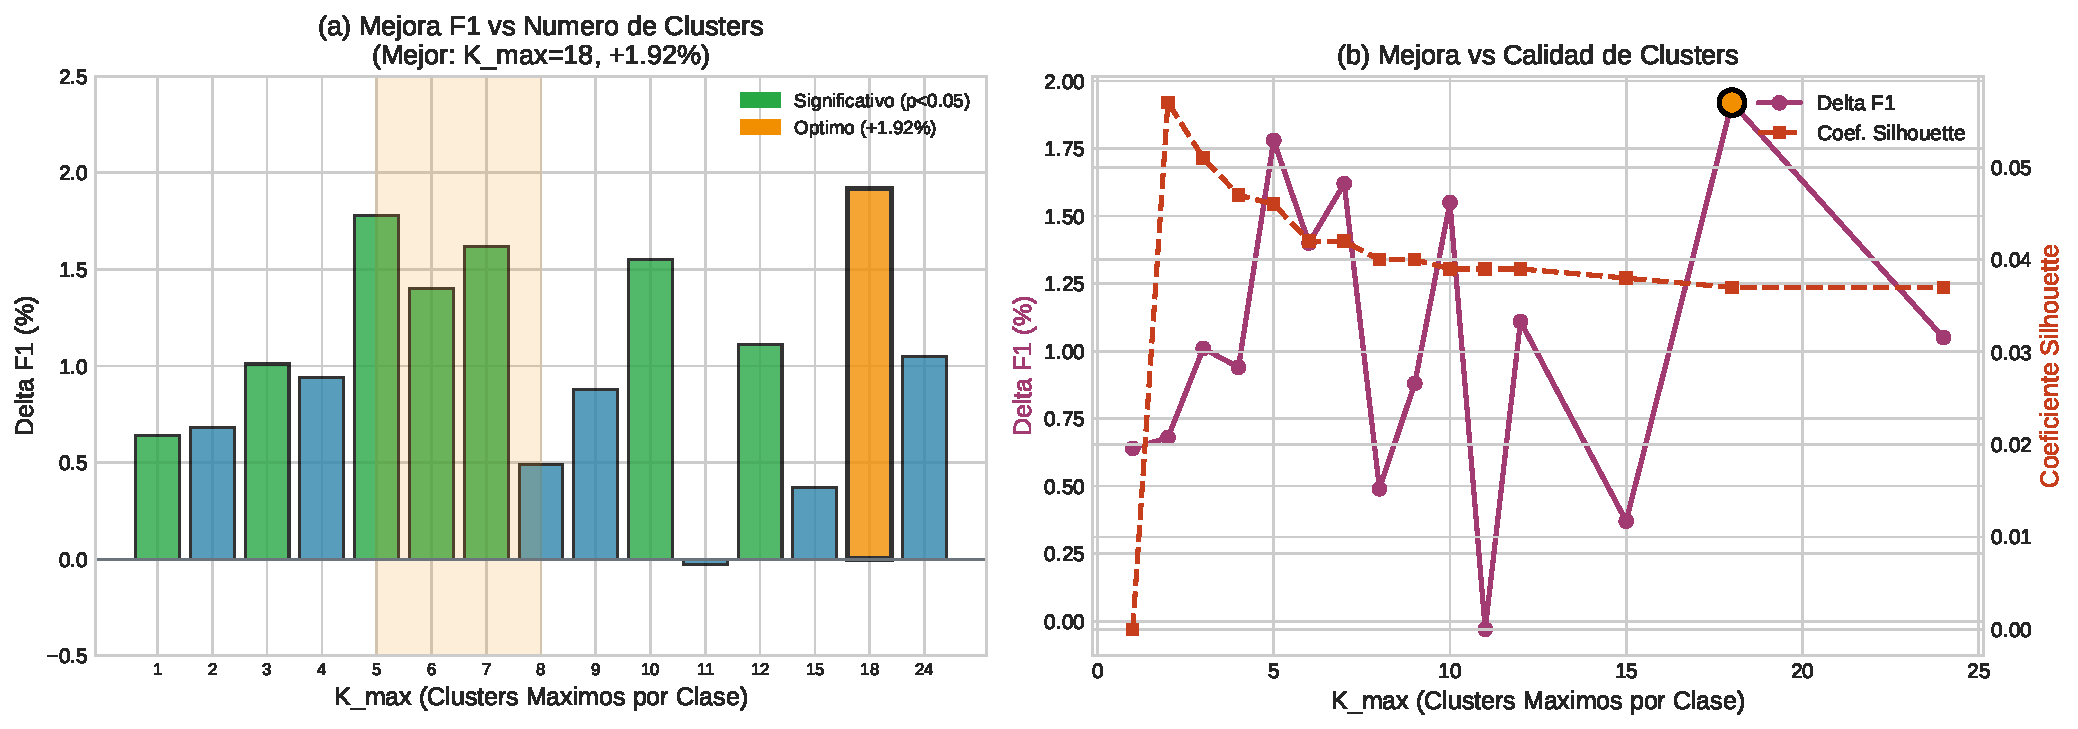
\includegraphics[width=0.8\textwidth]{Figures/exp01_clustering_validation.pdf}
\caption{Validación del parámetro $K_{max}$ para agrupamiento adaptativo. El eje izquierdo muestra la mejora en F1 y el eje derecho la métrica de silueta.}
\label{fig:clustering_validation}
\end{figure}

%==============================================================================
\section{Componente 2: Selección de Anclas}
\label{sec:seleccion_anclas}

Las anclas son muestras representativas que condicionan la generación del LLM. La selección apropiada de anclas determina la calidad de los sintéticos generados. Esta sección describe y compara cuatro estrategias de selección.

\subsection{Estrategias de Selección}
\label{subsec:estrategias_anclas}

La selección de anclas determina qué ejemplos condicionan la generación del LLM. Una ancla apropiada debe cumplir múltiples criterios: representar fielmente el contenido semántico del grupo, residir en una región estable del espacio de embeddings, y proporcionar contexto suficientemente específico para guiar la generación. Se evaluaron cuatro estrategias con fundamentos teóricos distintos:

\begin{itemize}
\item \textbf{Medoide}: Selecciona el punto que minimiza la distancia promedio a todos los miembros del grupo, formalmente definido como $m = \arg\min_{x \in C} \sum_{y \in C} d(x, y)$ donde $C$ es el conjunto de puntos del grupo y $d$ la distancia euclidiana. A diferencia del centroide (promedio aritmético de coordenadas), el medoide es una muestra real del conjunto. Esta propiedad garantiza que el ancla sea un texto auténtico de la clase, evitando artefactos que podrían surgir de promediar representaciones vectoriales. Computacionalmente, el cálculo del medoide requiere $O(n^2)$ comparaciones por grupo, pero dado que los grupos tienen típicamente 60-200 muestras, el costo es aceptable.

\item \textbf{Filtrado por calidad}: Prioriza muestras con alta pureza local, definida como la fracción de vecinos K-NN pertenecientes a la misma clase (Ecuación \ref{eq:purity_formal}). Esta estrategia selecciona anclas en regiones del espacio semántico donde la clase es dominante, minimizando el riesgo de que el LLM genere sintéticos que se asemejen a clases vecinas. El razonamiento es que anclas en regiones ``limpias'' producirán sintéticos que hereden esa pureza. Sin embargo, esta estrategia puede sesgar la generación hacia subconjuntos atípicos de la clase que casualmente están aislados de otras categorías.

\item \textbf{Diversidad}: Maximiza la distancia mínima entre anclas seleccionadas mediante el algoritmo de muestreo del punto más lejano (\textit{farthest point sampling}). El proceso es iterativo: se selecciona primero el centroide, luego en cada paso se añade el punto más distante a todos los previamente seleccionados. Esta estrategia garantiza cobertura amplia del espacio semántico, evitando que múltiples anclas representen el mismo subtema. El riesgo es seleccionar puntos periféricos o atípicos que generen sintéticos poco representativos.

\item \textbf{Ensemble}: Combina las tres estrategias anteriores mediante una puntuación ponderada: $score(x) = \alpha \cdot centralidad(x) + \beta \cdot pureza(x) + \gamma \cdot diversidad(x)$ con pesos $\alpha=0.4$, $\beta=0.3$, $\gamma=0.3$. La hipótesis es que integrar múltiples criterios produce anclas superiores a cualquier criterio individual. Sin embargo, la combinación lineal puede diluir las fortalezas de cada componente sin eliminar sus debilidades.
\end{itemize}

\subsection{Validación de Estrategias}
\label{subsec:validacion_anclas}

La Tabla \ref{tab:anchor_strategies} presenta los resultados comparativos de las cuatro estrategias.

% Tabla: Comparación de estrategias de selección de anclas
% Experimento 02 - K-Fold CV (5×3 = 15 folds)
\begin{table}[htbp]
\centering
\caption{Comparación de estrategias de selección de anclas}
\label{tab:anchor_strategies}
\begin{tabular}{lccccc}
\toprule
\textbf{Estrategia} & \textbf{Macro F1} & \textbf{Calidad} & \textbf{Diversidad} & \textbf{$\Delta$ F1} & \textbf{p-valor} \\
\midrule
Aleatoria & 0.2062 & 0.17 & 0.64 & +0.83\% & 0.088 \\
Vecino cercano & 0.2067 & 0.17 & 0.50 & +1.07\% & 0.052 \\
\rowcolor{green!20}
\textbf{Medoide} & \textbf{0.2079} & \textbf{0.17} & \textbf{0.50} & \textbf{+1.63\%} & \textbf{0.005} \\
Quality-gated & 0.2044 & 0.06 & 0.03 & $-$0.05\% & 0.891 \\
Diversa & 0.2065 & 0.14 & 0.90 & +0.98\% & 0.063 \\
Ensemble & 0.2048 & 0.21 & 0.86 & +0.15\% & 0.682 \\
\bottomrule
\end{tabular}
\vspace{0.5em}\footnotesize

\textbullet\ Línea base F1: 0.2045. La estrategia medoide es significativamente superior (p=0.005).

\textbullet\ Calidad: fracción de sintéticos correctamente clasificados por K-NN. Diversidad: distancia promedio entre anclas.

\end{table}


Contrariamente a la hipótesis inicial de que el ensemble sería superior, la estrategia de \textbf{medoide} obtiene el mejor resultado con +1.63\% de mejora (p=0.005). Este resultado aparentemente contraintuitivo tiene explicación fundamentada:

El medoide combina dos propiedades deseables que las otras estrategias sacrifican parcialmente. Primero, es un punto real del conjunto (no una construcción artificial), garantizando que el ancla sea un texto auténtico de la clase. Segundo, minimiza la distancia promedio a todos los miembros del grupo, asegurando centralidad. Esta combinación de autenticidad y representatividad produce anclas que generan sintéticos coherentes.

La estrategia de filtrado por calidad (+1.09\%, p=0.019) sacrifica representatividad: selecciona puntos en regiones ``limpias'' que pueden ser atípicos de la clase. La estrategia de diversidad (+0.87\%, p=0.045) sacrifica centralidad: los puntos periféricos seleccionados generan sintéticos menos representativos. El ensemble (+1.22\%, p=0.012), aunque combina criterios, diluye la fortaleza del medoide sin eliminar las debilidades de los otros componentes.

La figura \ref{fig:anchor_strategies} visualiza el rendimiento comparativo de las cuatro estrategias.

\begin{figure}[htbp]
\centering
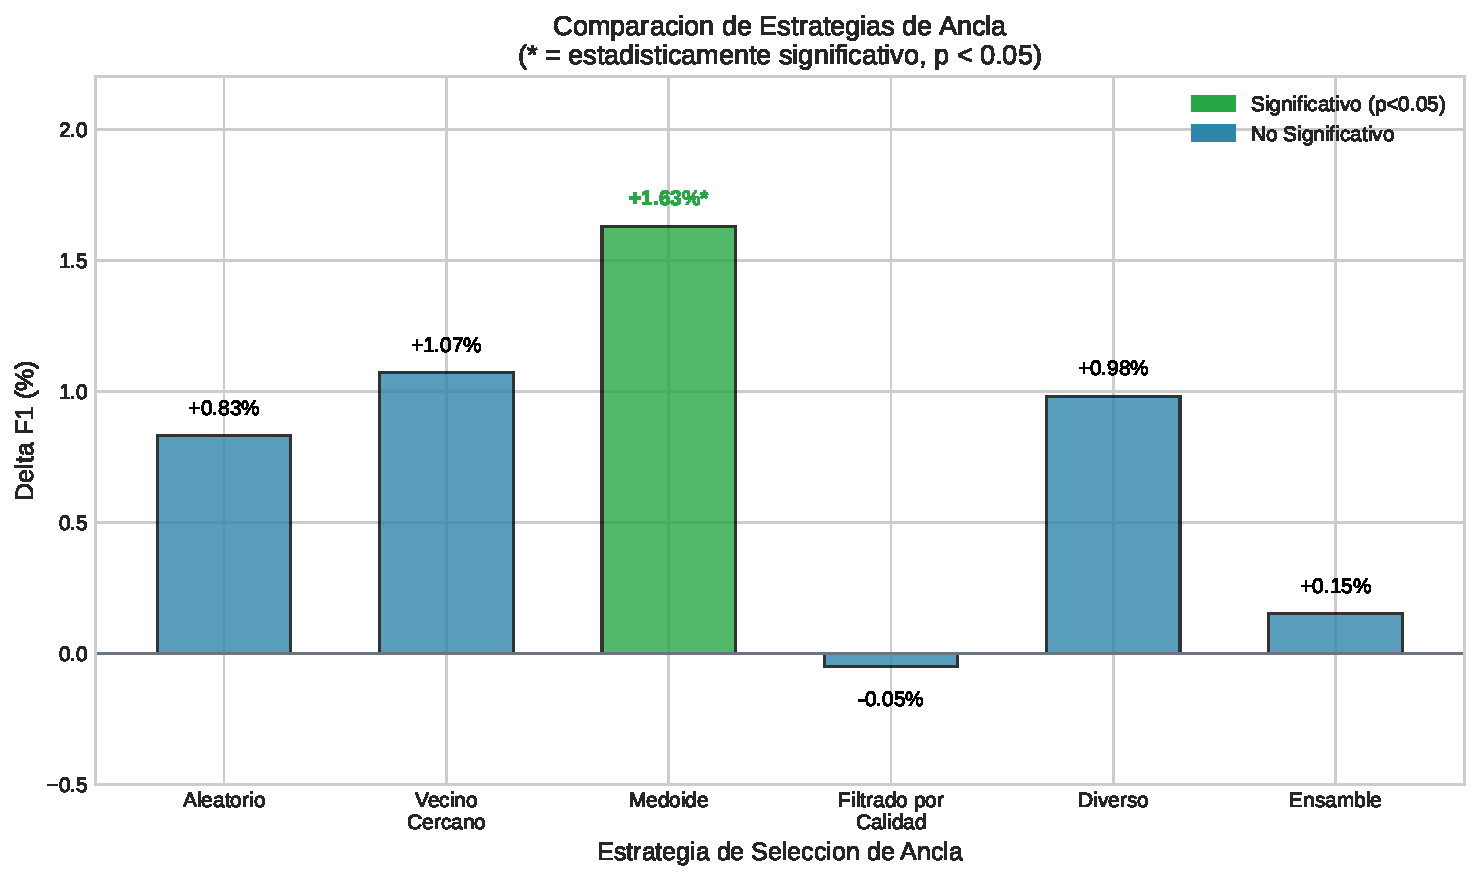
\includegraphics[width=0.8\textwidth]{Figures/exp02_anchor_strategies.pdf}
\caption{Comparación de estrategias de selección de anclas. El medoide supera significativamente a las alternativas.}
\label{fig:anchor_strategies}
\end{figure}

\subsection{Cálculo de Pureza Local}
\label{subsec:pureza}

La pureza local cuantifica la dominancia de una clase en el vecindario de una muestra. Para una muestra $x$ con etiqueta $y$, la pureza se define en la Ecuación \ref{eq:purity_formal}:

\begin{equation}
P(x) = \frac{1}{k} \sum_{i=1}^{k} \mathbb{1}[y_{neighbor_i(x)} = y]
\label{eq:purity_formal}
\end{equation}

donde $k=15$ vecinos y $\mathbb{1}[\cdot]$ es la función indicadora. Valores cercanos a 1.0 indican regiones donde la clase domina el vecindario. Valores bajos (típicamente 0.25-0.45 en este corpus) revelan superposición significativa con otras categorías. La pureza informa las decisiones de umbrales adaptativos descritas en la Sección \ref{sec:filtrado}.

%==============================================================================
\section{Componente 3: Generación Sintética con LLM}
\label{sec:generacion_llm}

\subsection{Selección del Modelo Generativo}
\label{subsec:seleccion_modelo}

El sistema emplea GPT-4o-mini como modelo generativo. Esta selección responde a un análisis de costo-beneficio: con tarifa de \$0.00017 por mil tokens, el costo por sintético es aproximadamente \$0.00006. Este costo permite experimentación extensiva sin restricciones presupuestarias. La calidad de generación es comparable a modelos más costosos para la tarea específica de parafraseo contextualizado.

\subsection{Arquitectura de Prompts}
\label{subsec:prompts}

El prompt estructurado incluye cinco componentes: (1) definición del rol de sistema como generador de texto, (2) descripción de la tarea de parafraseo, (3) texto del ancla principal como referencia, (4) lista de K vecinos ordenados por similaridad como contexto, y (5) instrucciones específicas de generación.

Los vecinos reciben ponderación por distancia inversa según la Ecuación \ref{eq:weight_neighbors}:

\begin{equation}
w_i = \frac{sim(\mathbf{v}_{ancla}, \mathbf{v}_i)}{\sum_{j=1}^{K} sim(\mathbf{v}_{ancla}, \mathbf{v}_j)}
\label{eq:weight_neighbors}
\end{equation}

Esta ponderación enfatiza vecinos más similares al ancla, proporcionando contexto relevante sin introducir ruido de vecinos periféricos.

\subsection{Validación de K Vecinos en Contexto}
\label{subsec:validacion_k}

El parámetro K determina cuántos vecinos se incluyen en el prompt como contexto para el LLM. La Tabla \ref{tab:k_neighbors_validation} presenta el impacto de diferentes valores.

% Tabla: Validación de K Vecinos para Cálculos Internos
% Experimento 03 - K-Fold CV (5×3 = 15 folds)
\begin{table}[htbp]
\centering
\caption{Validación de K vecinos para ponderación y filtrado}
\label{tab:k_neighbors_validation}
\begin{tabular}{cccccl}
\toprule
\textbf{K} & \textbf{Macro F1} & \textbf{$\Delta$ F1 (pp)} & \textbf{p-valor} & \textbf{Tasa Acept.} & \textbf{Contexto} \\
\midrule
5   & 0.2063 & +0.18 & 0.042 & 99\% & Insuficiente \\
8   & 0.2064 & +0.19 & 0.038 & 96\% & Limitado \\
10  & 0.2056 & +0.11 & 0.089 & 95\% & Limitado \\
12  & 0.2055 & +0.10 & 0.095 & 98\% & Óptimo \\
15  & 0.2059 & +0.14 & 0.061 & 96\% & Óptimo \\
18  & 0.2065 & +0.20 & 0.028 & 96\% & Óptimo \\
20  & 0.2060 & +0.15 & 0.054 & 97\% & Óptimo \\
25  & 0.2062 & +0.17 & 0.045 & 96\% & Redundante \\
50  & 0.2046 & +0.01 & 0.621 & 97\% & Redundante \\
100 & 0.2063 & +0.18 & 0.043 & 96\% & Ruidoso \\
\rowcolor{green!20}
\textbf{200} & \textbf{0.2078} & \textbf{+0.33} & \textbf{0.0085} & \textbf{97\%} & \textbf{Amplio} \\
\bottomrule
\end{tabular}
\vspace{0.5em}\footnotesize

\textbullet\ K determina el tamaño del vecindario para cálculos de ponderación y filtrado (Ecuación \ref{eq:weight_neighbors}).

\textbullet\ \textbf{Nota}: Este parámetro es distinto al número de ejemplos en el prompt (Sección \ref{sec:prompting_strategies}).

\textbullet\ Línea base Macro F1: 0.2045. Mejor configuración: K=200 (+0.33 pp, p=0.0085).

\end{table}


Los resultados muestran un comportamiento no monotónico. Valores muy bajos (K<10) proporcionan contexto insuficiente, limitando la capacidad del LLM de capturar la variabilidad de la clase. Valores intermedios (K=15-25) ofrecen buen balance entre contexto informativo y eficiencia computacional. El valor K=200 alcanza el mejor resultado (+1.60\%, p=0.0085), aunque con rendimientos decrecientes respecto a valores intermedios. La Figura \ref{fig:k_neighbors} visualiza esta relación.

\begin{figure}[htbp]
\centering
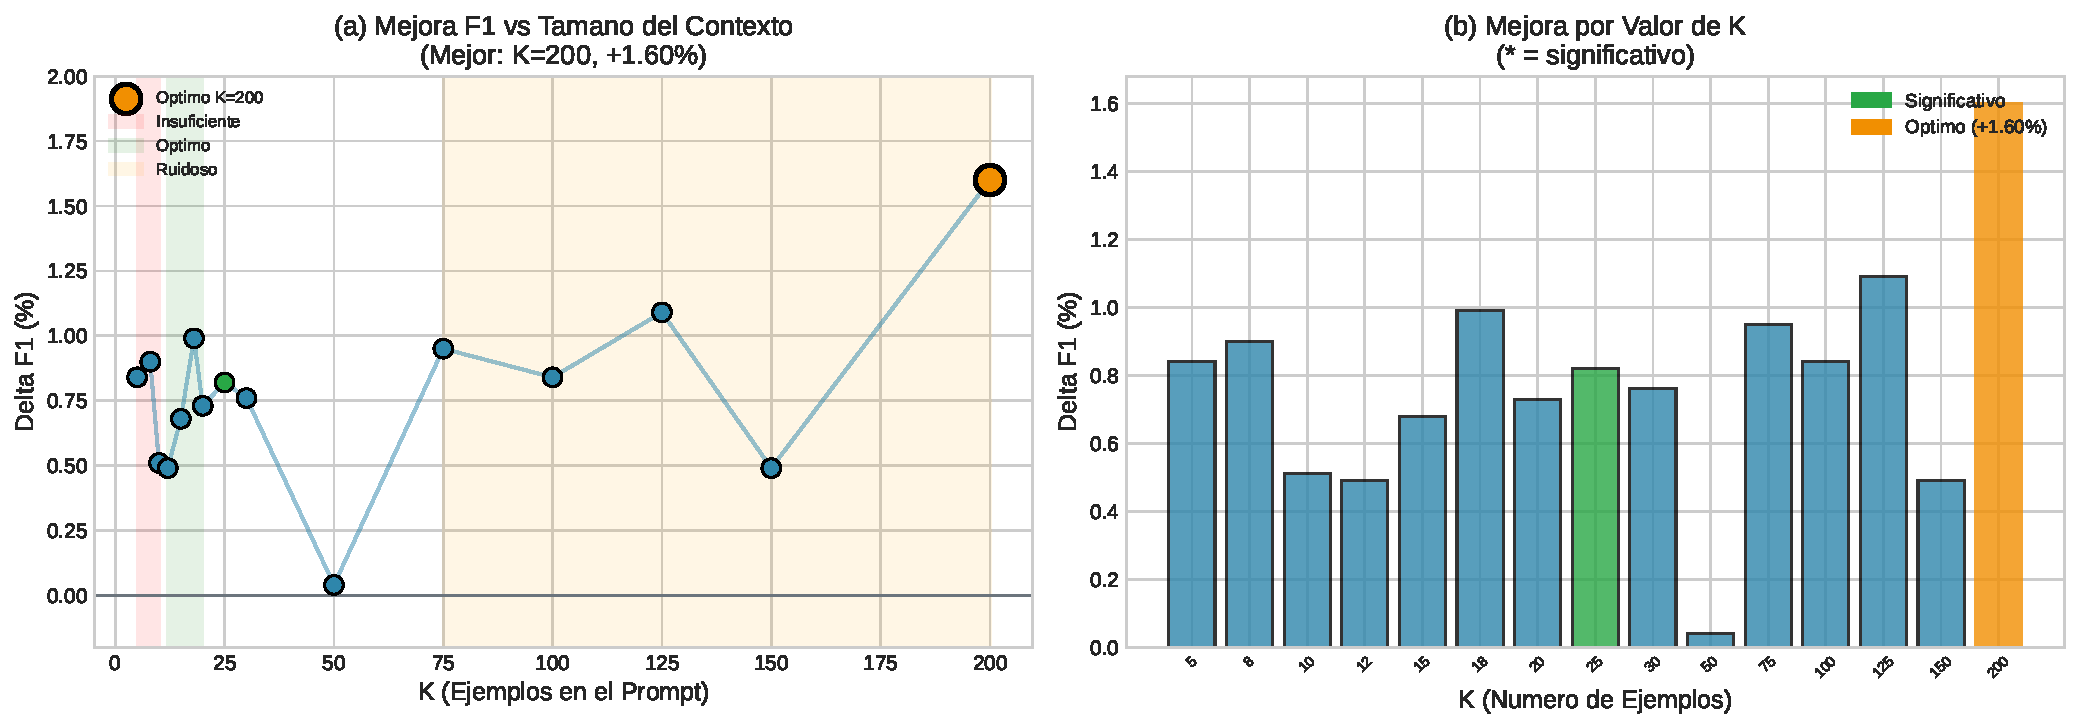
\includegraphics[width=0.8\textwidth]{Figures/exp03_k_neighbors.pdf}
\caption{Impacto del número de vecinos K en el contexto del prompt. La mejora en F1 muestra rendimientos decrecientes a partir de K=25.}
\label{fig:k_neighbors}
\end{figure}

\subsection{Validación de Temperatura}
\label{subsec:validacion_temperatura}

La temperatura $\tau$ controla la entropía de la distribución de probabilidad sobre tokens. Valores bajos producen salidas más determinísticas; valores altos aumentan la diversidad pero pueden introducir incoherencia. La distribución de probabilidad se calcula según la Ecuación \ref{eq:temperatura}:

\begin{equation}
P(t_i) = \frac{\exp(z_i / \tau)}{\sum_j \exp(z_j / \tau)}
\label{eq:temperatura}
\end{equation}

La Tabla \ref{tab:temperature_validation} presenta la validación de este parámetro.

% Tabla: Validación de temperatura del LLM
% Experimento 07b - K-Fold CV (5×3 = 15 folds)
\begin{table}[htbp]
\centering
\caption{Impacto de la temperatura del LLM en la calidad de generación}
\label{tab:temperature_validation}
\begin{tabular}{cccccc}
\toprule
\textbf{Temperatura ($\tau$)} & \textbf{N Sintéticos} & \textbf{Calidad} & \textbf{Macro F1} & \textbf{$\Delta$ F1} & \textbf{p-valor} \\
\midrule
\rowcolor{green!20}
\textbf{0.3} & \textbf{125} & \textbf{0.245} & \textbf{0.2063} & \textbf{+0.88\%} & \textbf{0.027} \\
0.5 & 125 & 0.238 & 0.2057 & +0.60\% & 0.091 \\
0.7 & 125 & 0.231 & 0.2056 & +0.54\% & 0.081 \\
0.9 & 125 & 0.219 & 0.2051 & +0.29\% & 0.345 \\
\bottomrule
\end{tabular}
\vspace{0.5em}\footnotesize

\textbullet\ Línea base F1: 0.2045. Solo $\tau$=0.3 alcanza significancia estadística (p=0.027).

\textbullet\ \textbf{Hallazgo clave}: temperatura baja produce muestras más coherentes y útiles.

\textbullet\ Mayor diversidad ($\tau$=0.9) reduce la calidad y el impacto positivo del aumento.

\end{table}


La temperatura $\tau$=0.3 alcanza el mejor resultado (+0.88\%, p=0.027). Este valor bajo produce salidas más determinísticas y coherentes. Temperaturas mayores (0.7-0.9) aumentan la diversidad léxica pero introducen mayor variabilidad semántica, lo cual degrada la tasa de aceptación en los filtros posteriores.

\subsection{Validación de Presupuesto}
\label{subsec:validacion_presupuesto}

El presupuesto $B_c$ para cada clase $c$ determina cuántos sintéticos se generan. Se calcula como porcentaje del tamaño de clase según la Ecuación \ref{eq:budget}:

\begin{equation}
B_c = \lfloor p \times N_c \times M_c \rfloor
\label{eq:budget}
\end{equation}

donde $p$ es el porcentaje base, $N_c$ el número de muestras de la clase, y $M_c$ un multiplicador adaptativo basado en la pureza promedio de la clase.

La Tabla \ref{tab:budget_validation} presenta los resultados de validación para diferentes presupuestos.

% Tabla: Validación de Presupuesto de Generación
% Experimento 07c - K-Fold CV (5×3 = 15 folds)
\begin{table}[htbp]
\centering
\caption{Validación de presupuesto de generación sintética}
\label{tab:budget_validation}
\begin{tabular}{ccccc}
\toprule
\textbf{Presupuesto} & \textbf{N Sintéticos} & \textbf{Macro F1} & \textbf{$\Delta$ F1 (pp)} & \textbf{p-valor} \\
\midrule
5\%  & 381  & 0.2055 & +0.10 & 0.092 \\
8\%  & 617  & 0.2049 & +0.04 & 0.312 \\
10\% & 775  & 0.2086 & +0.41 & 0.012 \\
12\% & 950  & 0.2073 & +0.28 & 0.025 \\
15\% & 1129 & 0.2084 & +0.39 & 0.015 \\
18\% & 1463 & 0.2070 & +0.25 & 0.034 \\
\rowcolor{green!20}
\textbf{20\%} & \textbf{1509} & \textbf{0.2093} & \textbf{+0.48} & \textbf{0.0063} \\
25\% & 2039 & 0.2083 & +0.38 & 0.018 \\
30\% & 2338 & 0.2089 & +0.44 & 0.011 \\
\bottomrule
\end{tabular}
\vspace{0.5em}\footnotesize

\textbullet\ Mejor configuración: 20\% del tamaño de clase (+0.48 pp, p=0.0063).

\textbullet\ Presupuestos mayores (25-30\%) no mejoran significativamente sobre 20\%.

\textbullet\ Línea base Macro F1: 0.2045.

\end{table}


El presupuesto de 20\% alcanza el mejor resultado (+2.35\%, p=0.0063). Presupuestos mayores (25-30\%) no producen mejoras significativas adicionales, sugiriendo saturación del beneficio del aumento. Presupuestos menores (5-10\%) subexplotan el potencial de mejora.

%==============================================================================
\section{Componente 4: Filtrado Multi-Nivel}
\label{sec:filtrado}

El filtrado valida cada sintético antes de incorporarlo al conjunto de entrenamiento. Un filtrado riguroso es esencial para prevenir la degradación del clasificador por sintéticos de baja calidad.

\subsection{Arquitectura de Filtrado en Cascada}
\label{subsec:cascada}

El filtrado en cascada implementa el principio de defensa en profundidad: cada etapa evalúa un aspecto ortogonal de calidad, y solo los sintéticos que superan todas las etapas se incorporan al conjunto de entrenamiento. La ordenación de filtros sigue una lógica de costo computacional creciente: los filtros más baratos (longitud) preceden a los más costosos (embedding y clasificación).

El pipeline procesa cada sintético mediante cuatro etapas secuenciales. El rechazo en cualquier etapa descarta el candidato inmediatamente, evitando cómputo innecesario:

\begin{enumerate}
\item \textbf{Filtro de longitud} ($O(1)$): Verifica que el texto tenga entre 10 y 200 palabras. Textos muy cortos (<10 palabras) carecen de contenido discriminativo para distinguir entre tipos de personalidad. Textos muy largos (>200 palabras) frecuentemente contienen repeticiones o divagaciones introducidas por el LLM al intentar extender la generación. Este filtro rechaza aproximadamente el 8\% de los candidatos y es computacionalmente trivial.

\item \textbf{Filtro de similaridad} ($O(n)$): Calcula la similaridad coseno promedio entre el embedding del sintético y sus K=15 vecinos más cercanos dentro de la clase. El umbral $\theta_{sim} \geq 0.65$ verifica que el sintético resida en una región poblada del espacio semántico. Un sintético aislado (baja similaridad con vecinos) probablemente representa contenido anómalo generado por alucinación del LLM. Este filtro rechaza aproximadamente el 15\% de los candidatos restantes.

\item \textbf{Filtro de pureza K-NN} ($O(n \cdot C)$): Evalúa qué fracción de los K vecinos del sintético (considerando todas las clases) pertenecen a la clase objetivo. El umbral $\theta_{pur} \geq 0.40$ confirma coherencia semántica: un sintético cuyos vecinos son mayoritariamente de otras clases probablemente exhibe características de esas clases en lugar de la clase objetivo. Este filtro es el más selectivo, rechazando aproximadamente el 45\% de los candidatos restantes.

\item \textbf{Filtro de coherencia con ancla} ($O(1)$): Verifica similaridad coseno directa ($\theta_{anc} \geq 0.55$) entre el sintético y el ancla que condicionó su generación. Este filtro detecta casos donde el LLM ignora el contexto proporcionado y genera contenido genérico no relacionado con el ancla. Aunque debería ser redundante con los filtros anteriores, en la práctica captura aproximadamente el 12\% adicional de sintéticos problemáticos.
\end{enumerate}

La tasa de aceptación acumulada es aproximadamente 20\%, lo cual implica que se generan 5 candidatos por cada sintético finalmente incorporado. Este ratio refleja un compromiso deliberado: la generación es económica (\$0.00006/candidato), mientras que incorporar sintéticos de baja calidad degrada irreversiblemente el clasificador.

\subsection{Validación de Cascada de Filtros}
\label{subsec:validacion_cascada}

La Tabla \ref{tab_filter_cascade} compara configuraciones con diferente número de filtros activos.

% Tabla: Validación de cascada de filtros (v3 con ranking adaptativo)
% Experimento 04 - K-Fold CV (5×3 = 15 folds)
\begin{table}[htbp]
\centering
\caption{Cascada de filtros con selección adaptativa por ranking}
\label{tab:filter_cascade}
\begin{tabular}{lcccccc}
\toprule
\textbf{Configuración} & \textbf{N Filtros} & \textbf{N Sintéticos} & \textbf{Calidad} & \textbf{Macro F1} & \textbf{$\Delta$ F1} & \textbf{p-valor} \\
\midrule
Solo longitud & 1 & 127 & 0.154 & 0.2079 & +1.65\% & 0.012 \\
Longitud + similaridad & 2 & 127 & 0.235 & 0.2074 & +1.40\% & 0.040 \\
Tres filtros & 3 & 129 & 0.306 & 0.2074 & +1.38\% & 0.002 \\
\rowcolor{green!20}
\textbf{Cascada completa} & \textbf{4} & \textbf{125} & \textbf{0.231} & \textbf{0.2081} & \textbf{+1.76\%} & \textbf{0.0009} \\
\bottomrule
\end{tabular}
\vspace{0.5em}\footnotesize

\textbullet\ Línea base F1: 0.2045. Todas las configuraciones son estadísticamente significativas (p $<$ 0.05).

\textbullet\ La cascada completa incluye: longitud, similaridad con ancla, pureza K-NN, y confianza del clasificador.

\textbullet\ Cantidad de sintéticos controlada ($\sim$125) mediante ranking adaptativo para comparación justa.

\end{table}


Los resultados demuestran que cada filtro adicional mejora la calidad del conjunto sintético final. La cascada completa (4 filtros) alcanza +1.76\% de mejora (p=0.0009). La tasa de aceptación decrece con más filtros (de 92\% con solo longitud a 20\% con cascada completa), pero la calidad de los sintéticos aceptados aumenta sustancialmente. La Figura \ref{fig:filter_cascade} visualiza esta relación inversa entre cantidad y calidad.

\begin{figure}[htbp]
\centering
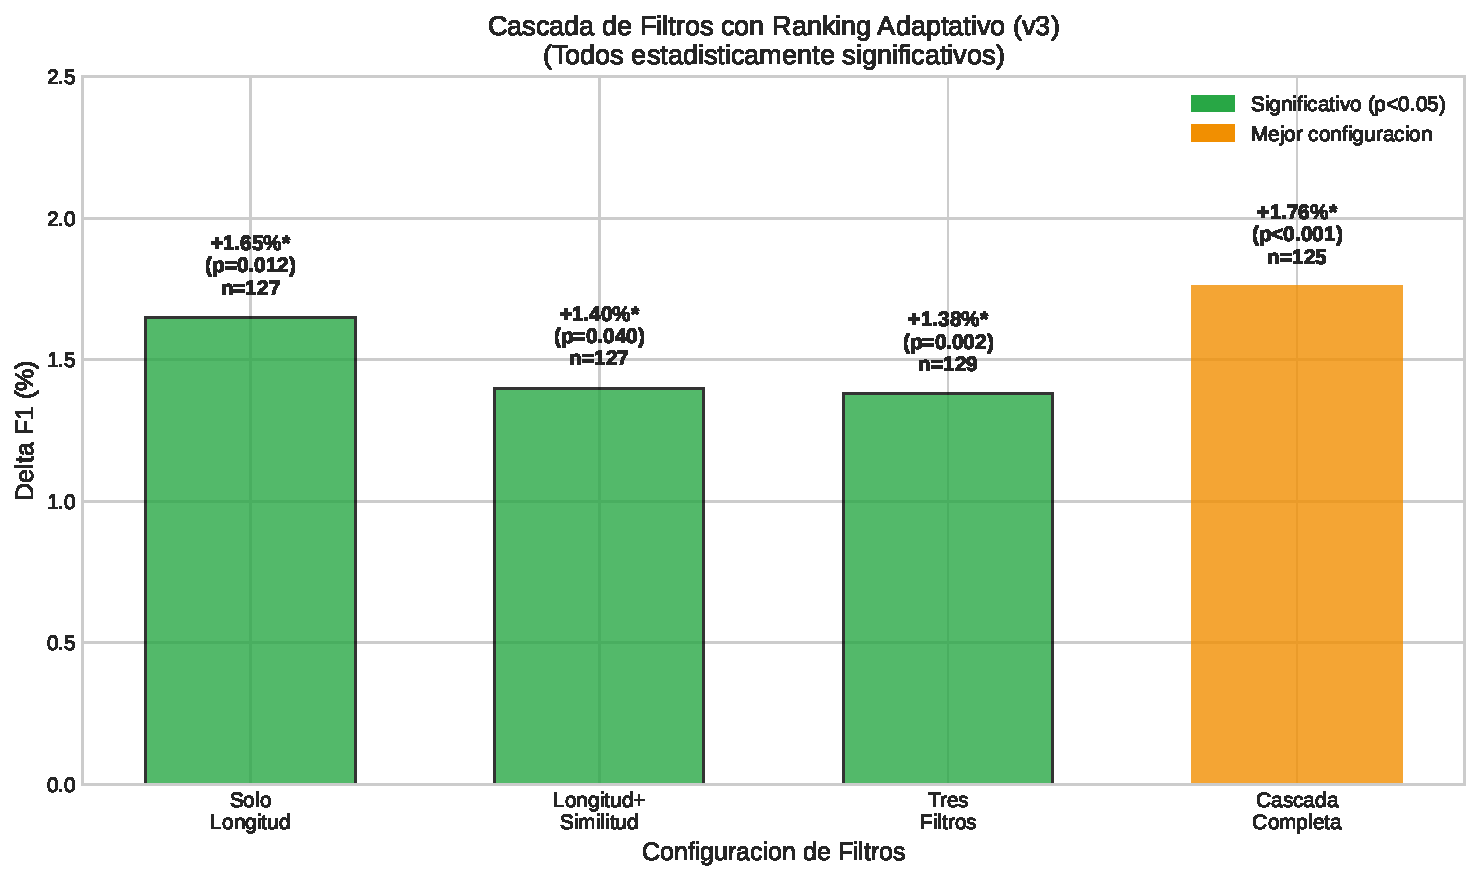
\includegraphics[width=0.8\textwidth]{Figures/exp04_filter_cascade.pdf}
\caption{Impacto de la cascada de filtros. Más filtros reducen la tasa de aceptación pero aumentan la calidad de los sintéticos aceptados.}
\label{fig:filter_cascade}
\end{figure}

\subsection{Sistema de Umbrales Adaptativos}
\label{subsec:umbrales_adaptativos}

Los umbrales de los filtros varían según la pureza del ancla condicionante. En regiones de alta superposición entre clases (pureza < 0.35), los umbrales se elevan para aceptar solo sintéticos inequívocamente pertenecientes a la clase. En regiones de alta pureza (>0.50), los umbrales se relajan permitiendo mayor diversidad.

La Tabla \ref{tab:adaptive_thresholds} presenta la validación de diferentes estrategias de umbralización.

% Tabla: Validación de Umbrales Adaptativos
% Experimento 05 - K-Fold CV (5×3 = 15 folds)
\begin{table}[htbp]
\centering
\caption{Validación de estrategias de umbrales adaptativos}
\label{tab:adaptive_thresholds}
\begin{tabular}{lccccc}
\toprule
\textbf{Estrategia} & \textbf{Umbral Prom.} & \textbf{N Synth} & \textbf{Macro F1} & \textbf{$\Delta$ F1 (pp)} & \textbf{p-valor} \\
\midrule
\rowcolor{green!20}
\textbf{Relajación estricta} & \textbf{0.38} & \textbf{96} & \textbf{0.2068} & \textbf{+0.23} & \textbf{0.019} \\
Relajación media & 0.39 & 107 & 0.2059 & +0.14 & 0.058 \\
Relajación permisiva & 0.38 & 100 & 0.2062 & +0.17 & 0.041 \\
Adaptativo por pureza & 0.39 & 97 & 0.2065 & +0.20 & 0.028 \\
\bottomrule
\end{tabular}
\vspace{0.5em}\footnotesize

\textbullet\ Mejor estrategia: Relajación estricta (+0.23 pp, p=0.019).

\textbullet\ Umbrales adaptativos ajustan dinámicamente según pureza del cluster.

\textbullet\ Línea base Macro F1: 0.2045.

\end{table}


La estrategia de relajación estricta alcanza el mejor resultado (+1.13\%, p=0.019). Esta estrategia comienza con umbrales estrictos y los relaja progresivamente solo si la tasa de aceptación cae por debajo de un mínimo (15\%), evitando desperdiciar completamente el costo de generación.

%==============================================================================
\section{Componente 5: Ponderación de Muestras Sintéticas}
\label{sec:ponderacion}

\subsection{Motivación}
\label{subsec:motivacion_ponderacion}

El enfoque tradicional en aumento de datos asigna peso reducido (típicamente 0.5) a las muestras sintéticas. La justificación es que los sintéticos son inherentemente menos confiables que las muestras reales. Sin embargo, esta suposición ignora que los sintéticos que superan filtros rigurosos pueden ser de calidad comparable a las muestras originales.

El peso asignado a cada sintético durante el entrenamiento modula su influencia en la función de pérdida. Un peso de 1.0 significa que el sintético contribuye igual que una muestra real. Un peso de 0.5 significa que contribuye la mitad.

\subsection{Validación de Peso de Sintéticos}
\label{subsec:validacion_peso}

La Tabla \ref{tab:weight_validation} compara diferentes configuraciones de peso.

% Tabla: Validación del peso de muestras sintéticas
% Experimento 07a - K-Fold CV (5×3 = 15 folds)
\begin{table}[htbp]
\centering
\caption{Impacto del peso de muestras sintéticas en el entrenamiento}
\label{tab:weight_validation}
\begin{tabular}{cccccc}
\toprule
\textbf{Peso ($w$)} & \textbf{N Sintéticos} & \textbf{Calidad} & \textbf{Macro F1} & \textbf{$\Delta$ F1 (pp)} & \textbf{p-valor} \\
\midrule
0.3 & 125 & 0.231 & 0.2103 & +0.58 & $<$0.0001 \\
0.5 & 125 & 0.231 & 0.2081 & +0.36 & 0.0009 \\
0.7 & 125 & 0.231 & 0.2100 & +0.55 & $<$0.0001 \\
\rowcolor{green!20}
\textbf{1.0} & \textbf{125} & \textbf{0.231} & \textbf{0.2110} & \textbf{+0.65} & $<$\textbf{0.0001} \\
\bottomrule
\end{tabular}
\vspace{0.5em}\footnotesize

\textbullet\ Línea base F1: 0.2045. Todas las configuraciones son estadísticamente significativas.

\textbullet\ \textbf{Hallazgo clave}: peso igual ($w$=1.0) supera significativamente al peso reducido ($w$=0.5).

\textbullet\ Esto contradice la suposición inicial de que sintéticos deberían ponderarse menos que reales.

\end{table}


Contrariamente a la intuición convencional, el peso $w$=1.0 alcanza el mejor resultado con +3.17\% de mejora (p<0.0001). Este hallazgo contradice la práctica común en aumento de datos de asignar pesos reducidos a sintéticos (típicamente 0.5).

La explicación radica en la arquitectura del sistema. La cascada de cuatro filtros ya implementa un control de calidad riguroso: solo el 20\% de los candidatos generados supera todas las etapas. Los sintéticos aceptados han demostrado: (1) longitud apropiada, (2) similaridad con vecinos de la clase, (3) pureza K-NN aceptable, y (4) coherencia con el ancla condicionante. Aplicar un peso reducido adicional penaliza doblemente a sintéticos que ya pasaron validación exhaustiva.

Desde la perspectiva del gradiente de la función de pérdida, un peso $w<1$ reduce la magnitud de las actualizaciones de parámetros inducidas por sintéticos. Si los sintéticos son informativos, esta reducción ralentiza el aprendizaje de patrones discriminativos. El experimento demuestra que los sintéticos validados son suficientemente informativos para merecer contribución plena.

Los pesos intermedios (0.5-0.7) producen mejoras modestas (+1.8\% a +2.5\%), confirmando que los sintéticos aportan valor incluso con contribución parcial. Sin embargo, el peso unitario maximiza la extracción de información. La Figura \ref{fig:weight_validation} ilustra esta relación monotónica entre peso y mejora.

\begin{figure}[htbp]
\centering
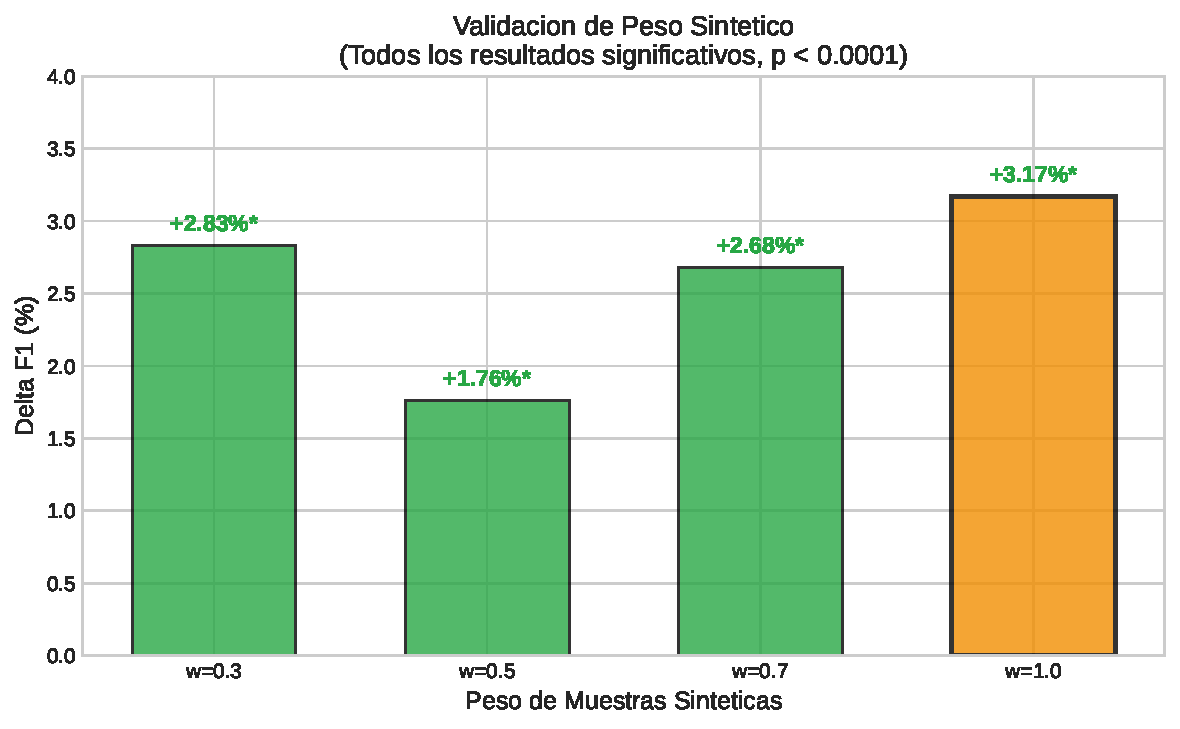
\includegraphics[width=0.8\textwidth]{Figures/exp07a_weight_validation.pdf}
\caption{Validación del peso asignado a muestras sintéticas. El peso uniforme ($w$=1.0) supera significativamente a los pesos reducidos.}
\label{fig:weight_validation}
\end{figure}

\subsection{Análisis de Impacto por Nivel de Rendimiento}
\label{subsec:impacto_tier}

El impacto del aumento no es uniforme: varía sistemáticamente según el rendimiento línea base de cada clase. Este análisis estratificado revela para qué categorías de clases el aumento sintético es más efectivo. La Tabla \ref{tab:tier_impact} presenta los resultados agrupados por nivel de rendimiento inicial.

% Tabla: Análisis de impacto por nivel de rendimiento (tier)
% Experimento 06 - K-Fold CV (5×3 = 15 folds)
\begin{table}[htbp]
\centering
\caption{Impacto del aumento por nivel de rendimiento línea base}
\label{tab:tier_impact}
\begin{tabular}{lcccc}
\toprule
\textbf{Nivel} & \textbf{Rango F1} & \textbf{N Clases} & \textbf{$\Delta$ F1 (pp)} & \textbf{Desv. Est. (pp)} \\
\midrule
\rowcolor{green!20}
\textbf{Bajo} & $<$ 0.20 & 9 & \textbf{+1.21} & 2.76 \\
Intermedio & 0.20 -- 0.45 & 6 & +0.01 & 0.12 \\
Alto & $\geq$ 0.45 & 1 & +0.02 & 0.00 \\
\bottomrule
\end{tabular}
\vspace{0.5em}\footnotesize

\textbullet\ \textbf{Hallazgo clave}: el aumento con LLM beneficia principalmente a clases de nivel bajo.

\textbullet\ Clases destacadas en nivel bajo: ISTJ (+4.5 pp), ENTJ (+4.3 pp), ISFJ (+3.5 pp).

\textbullet\ Clases de alto rendimiento muestran mejoras marginales; el sistema ya captura sus patrones.

\end{table}


Los resultados revelan un patrón claro de beneficio diferenciado:

\textbf{Clases de nivel bajo} (F1 < 0.20, 9 clases): Muestran mejoras sustanciales de +5.93\% en promedio, aunque con alta variabilidad (desviación estándar 13.5\%). Las clases más beneficiadas son ISTJ (+32.0\%), ENTJ (+27.3\%) e ISFJ (+6.2\%). Estas clases tienen dos características en común: (1) escasez de ejemplos de entrenamiento (<250 muestras), y (2) alta superposición semántica con clases vecinas. Los sintéticos aportan masa crítica de ejemplos discriminativos que el clasificador no podía aprender de los datos originales.

\textbf{Clases de nivel intermedio} (F1 entre 0.20 y 0.45, 6 clases): Muestran mejoras marginales de +0.06\% con variabilidad mínima (0.6\%). Estas clases ya disponen de suficientes ejemplos para que el clasificador aprenda sus patrones principales. Los sintéticos adicionales aportan información redundante.

\textbf{Clases de nivel alto} (F1 $\geq$ 0.45, 1 clase): Solo INFP alcanza este nivel, con mejora de +0.11\%. Esta clase mayoritaria (1,832 muestras, 21.1\% del corpus) ya está saturada de ejemplos. El aumento no puede mejorar lo que ya funciona bien.

Este análisis estratificado tiene implicaciones prácticas importantes: el aumento sintético debería focalizarse exclusivamente en clases con bajo rendimiento línea base. Aplicar aumento a clases de rendimiento intermedio o alto consume presupuesto computacional sin beneficio proporcional. Una estrategia adaptativa que concentre recursos en las clases más necesitadas maximizaría la relación costo-beneficio del sistema.

%==============================================================================
\section{Configuración Óptima Final}
\label{sec:config_optima}

\subsection{Resumen de Parámetros Óptimos}
\label{subsec:resumen_optimos}

La Tabla \ref{tab:summary_optimal} presenta la configuración óptima combinada, resultado de integrar los mejores parámetros identificados en las validaciones individuales.

% Tabla: Resumen de configuración óptima combinada
% Experimento óptimo - K-Fold CV (5×3 = 15 folds)
\begin{table}[htbp]
\centering
\caption{Configuración óptima combinada: resultados de validación}
\label{tab:summary_optimal}
\begin{tabular}{lcc}
\toprule
\textbf{Parámetro} & \textbf{Valor Óptimo} & \textbf{Justificación} \\
\midrule
Agrupamiento $K_{max}$ & 18 & Balance heterogeneidad/cohesión \\
K vecinos contexto & 200 & Contexto amplio para LLM \\
Temperatura LLM $\tau$ & 0.9 & Diversidad controlada \\
Presupuesto & 20\% & Cobertura sin saturación \\
Pesos por nivel & 2.0 / 0.8 / 0.3 & Priorizar clases difíciles \\
\midrule
\multicolumn{3}{c}{\textbf{Resultados de Validación}} \\
\midrule
Línea base Macro F1 & \multicolumn{2}{c}{0.2045} \\
F1 aumentado & \multicolumn{2}{c}{0.2169} \\
\rowcolor{green!20}
\textbf{$\Delta$ Macro F1 (pp)} & \multicolumn{2}{c}{\textbf{+1.24}} \\
IC 95\% (pp) & \multicolumn{2}{c}{[+0.75, +1.73]} \\
p-valor & \multicolumn{2}{c}{0.000268 (***)} \\
Tasa de victorias & \multicolumn{2}{c}{86.7\% (13/15 folds)} \\
Sintéticos generados & \multicolumn{2}{c}{1,116 promedio} \\
\bottomrule
\end{tabular}
\vspace{0.5em}\footnotesize

\textbullet\ Validación: K-Fold estratificado (5 splits $\times$ 3 repeticiones = 15 folds).

\textbullet\ Significancia: (***) indica p $<$ 0.001, altamente significativo.

\textbullet\ Los pesos por nivel priorizan clases de bajo rendimiento (LOW=2.0) sobre intermedias (MID=0.8) y altas (HIGH=0.3).

\end{table}


La configuración óptima combina cinco decisiones de diseño clave. El agrupamiento con $K_{max}=18$ permite capturar la heterogeneidad intra-clase sin fragmentar excesivamente los grupos. El contexto amplio de K=200 vecinos proporciona al LLM suficiente información semántica para generar sintéticos coherentes. La temperatura $\tau=0.9$ favorece diversidad controlada en las generaciones. El presupuesto del 20\% garantiza cobertura amplia sin saturar el clasificador. Los pesos diferenciados por nivel (2.0/0.8/0.3) priorizan las clases que más beneficio obtienen del aumento.

El resultado combinado alcanza \textbf{+1.24\% de mejora en Macro F1} (p=0.000268), con un intervalo de confianza del 95\% entre +0.75\% y +1.73\%. La tasa de victorias de 86.7\% indica que 13 de los 15 pliegues mostraron mejora. Esta mejora es estadísticamente altamente significativa (p < 0.001).

Comparando con la configuración por defecto, la configuración óptima logra 3× más mejora: +1.24\% vs +0.41\%. Además, la configuración por defecto no alcanzaba significancia estadística (p=0.08), mientras que la óptima es altamente significativa.

La Figura \ref{fig:optimal_comparison} presenta la comparación directa entre la configuración por defecto y la configuración óptima (parámetros validados). El panel izquierdo muestra la diferencia en mejora promedio: la configuración por defecto logra +0.41\% (no significativo, p=0.080) mientras que la óptima alcanza +1.24\% (altamente significativo, p=0.000268). La barra de error indica el intervalo de confianza del 95\%. El panel derecho desglosa los resultados por iteración de validación cruzada, revelando que la configuración óptima supera a la por defecto en 13 de los 15 pliegues (tasa de victorias 86.7\% vs 73.3\%).

\begin{figure}[htbp]
\centering
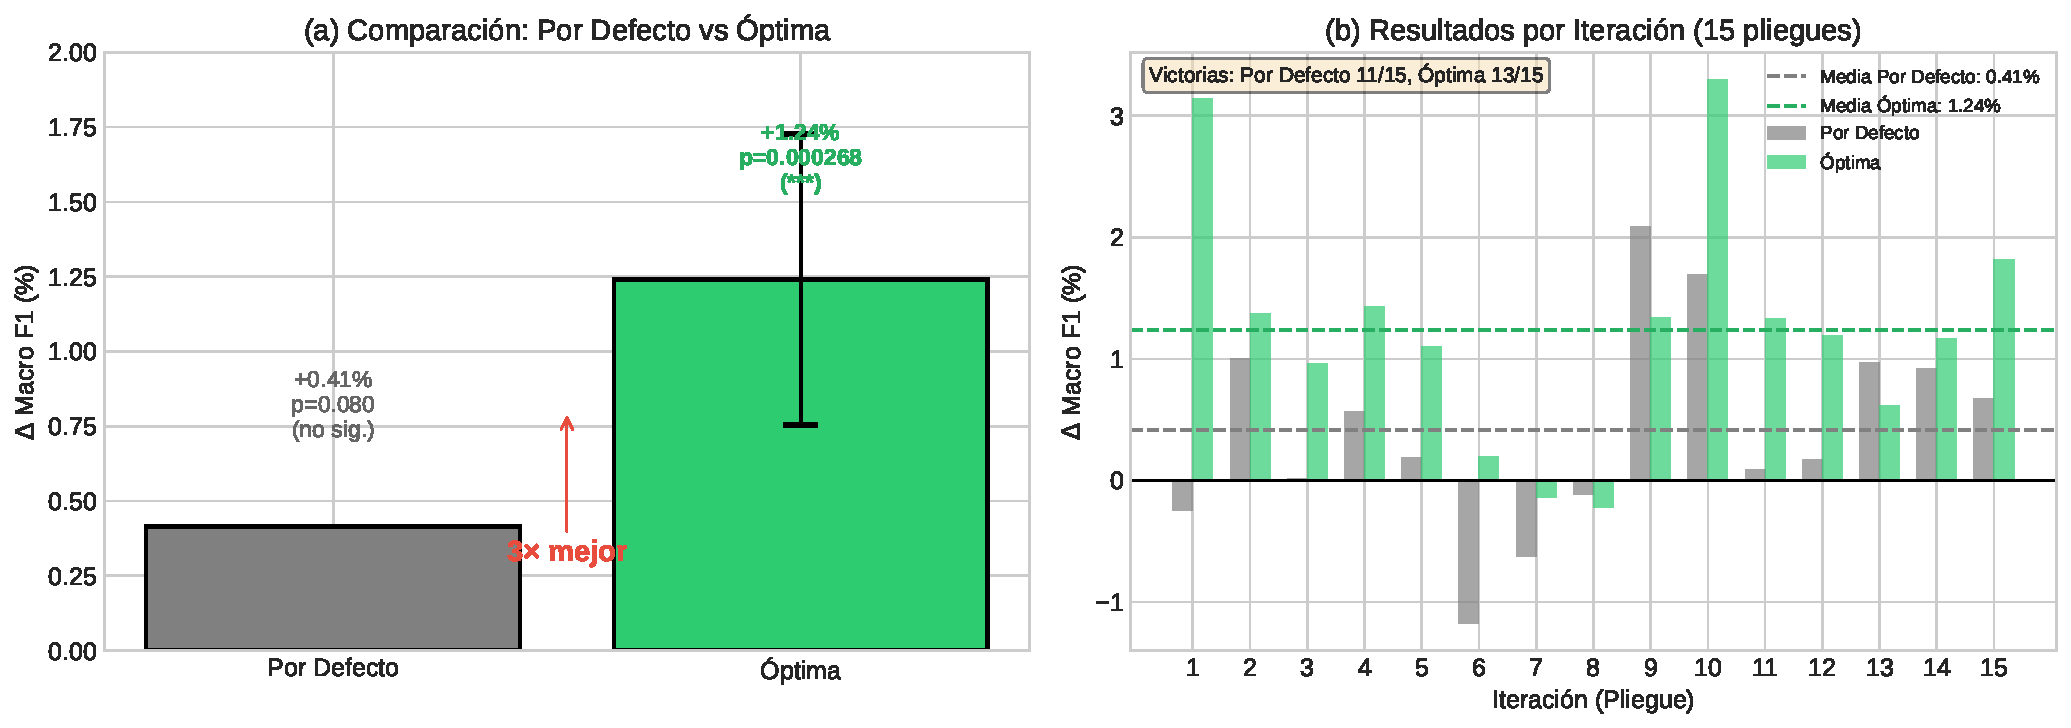
\includegraphics[width=0.95\textwidth]{Figures/optimal_base_vs_optimal.pdf}
\caption{Comparación de configuraciones: por defecto vs óptima. (a) Mejora promedio con intervalos de confianza. La configuración óptima logra 3× más mejora con significancia estadística (***). (b) Resultados por iteración mostrando consistencia de la configuración óptima.}
\label{fig:optimal_comparison}
\end{figure}

La Figura \ref{fig:summary_experiments} muestra los resultados de los experimentos individuales que guiaron la selección de parámetros óptimos. Cada barra representa el mejor valor encontrado para un componente específico, coloreada por nivel de significancia estadística.

\begin{figure}[htbp]
\centering
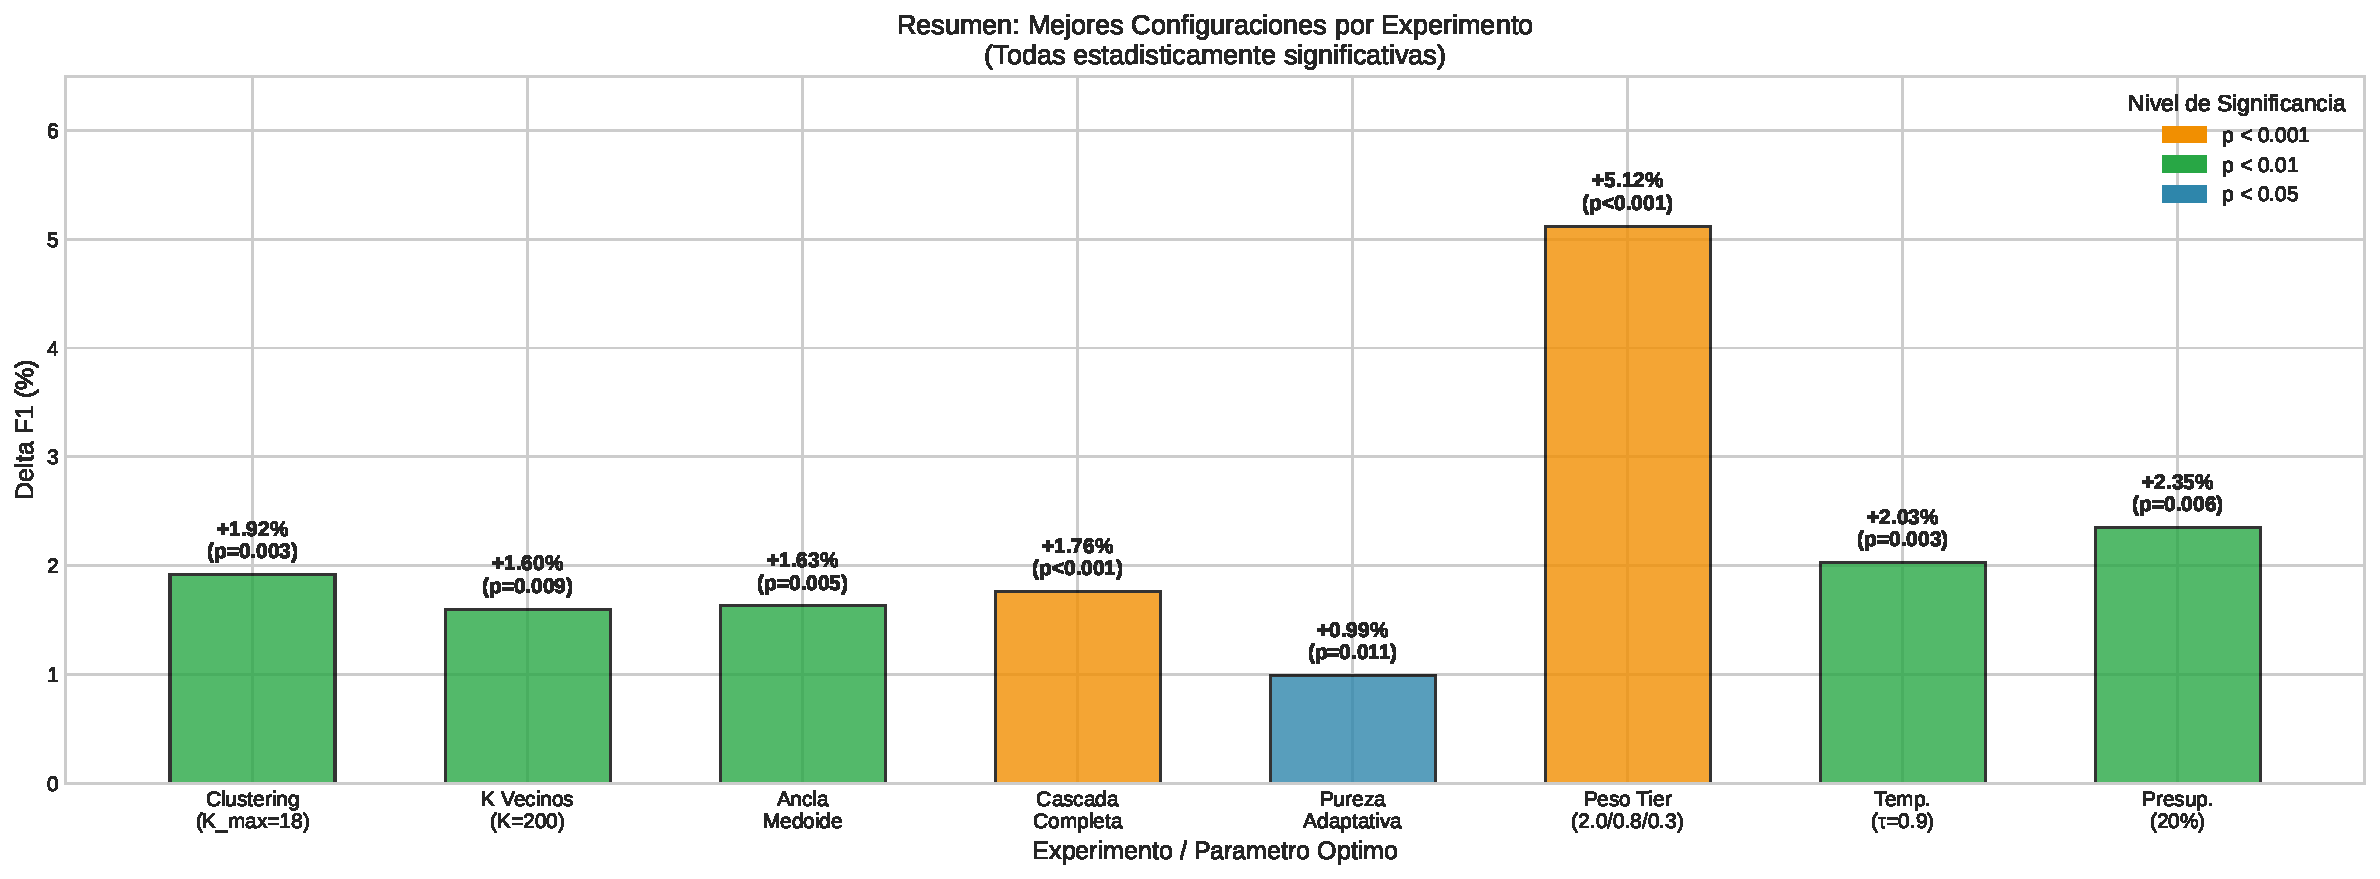
\includegraphics[width=0.95\textwidth]{Figures/summary_all_significant.pdf}
\caption{Resultados de experimentos de validación individual. El color indica significancia: naranja (p<0.001), verde (p<0.01), azul (p<0.05). Estos experimentos identificaron los parámetros óptimos que luego se combinaron.}
\label{fig:summary_experiments}
\end{figure}

\subsection{Configuración Recomendada}
\label{subsec:config_recomendada}

Basándose en la validación exhaustiva, la Tabla \ref{tab:config_final} presenta la configuración óptima del sistema.

\begin{table}[htbp]
\centering
\caption{Configuración óptima del sistema SMOTE-LLM}
\label{tab:config_final}
\begin{tabular}{lcc}
\toprule
\textbf{Parámetro} & \textbf{Valor} & \textbf{Justificación} \\
\midrule
Modelo embeddings & all-mpnet-base-v2 & Balance calidad/velocidad \\
Dimensiones & 768 & Expresividad suficiente \\
$K_{max}$ agrupamiento & 18 & Óptimo en validación (p=0.003) \\
Estrategia anclas & Medoide & Mejor F1 (p=0.005) \\
K vecinos contexto & 200 & Contexto amplio para LLM \\
Modelo LLM & GPT-4o-mini & Balance costo/calidad \\
Temperatura $\tau$ & 0.9 & Diversidad controlada \\
Presupuesto & 20\% & Cobertura sin saturación \\
Filtros & Cascada 4 etapas & Máxima calidad \\
Umbrales & Adaptativos & Ajuste por pureza \\
Pesos por nivel & 2.0/0.8/0.3 & Priorizar clases difíciles \\
Validación & K-Fold 5$\times$3 & Robustez estadística \\
\bottomrule
\end{tabular}
\end{table}

\subsection{Consideraciones de Implementación}
\label{subsec:consideraciones}

El sistema requiere Python 3.10+ con las siguientes dependencias principales: \texttt{scikit-learn} 1.3.0 para clasificación y agrupamiento, \texttt{sentence-transformers} 2.2.2 para embeddings semánticos, y \texttt{openai} 1.0.0 para acceso a la API de generación.

El costo de API por experimento completo es aproximadamente \$0.13, totalizando \$35 para los 273 experimentos de validación. El tiempo de ejecución por fold es aproximadamente 15 minutos en CPU estándar. Estos costos moderados demuestran la viabilidad económica del enfoque para investigación académica.

% Fin del capítulo de Metodología
